% Copyright (C) 2010,2011,2012,2013 The ESPResSo project
%  
% This file is part of ESPResSo.
%   
% ESPResSo is free software: you can redistribute it and/or modify it
% under the terms of the GNU General Public License as published by the
% Free Software Foundation, either version 3 of the License, or (at your
% option) any later version.
%  
% ESPResSo is distributed in the hope that it will be useful, but
% WITHOUT ANY WARRANTY; without even the implied warranty of
% MERCHANTABILITY or FITNESS FOR A PARTICULAR PURPOSE.  See the GNU
% General Public License for more details.
%  
% You should have received a copy of the GNU General Public License
% along with this program.  If not, see <http://www.gnu.org/licenses/>.
%

\chapter{Object-in-fluid}
\label{sec:fsi}
\newescommand{fsi}

\begin{citebox}
  Please cite~\citewbibkey{cimrak} if you use the object-in-fluid implementation described below.
\end{citebox}


Simulations using \es work mostly with objects (molecules, atoms, 
polymers, colloids, crystals, ...) that are physicaly composed of points linked 
together with bonds. These objects are like skeletons, without inner or outer volume. 

The idea is to use \es for objects that do have inner volume, for example blood cells, 
magnetic beads, capsules, ... The boundary of an object is covered with triangular 
mesh. The vertices of the mesh are put into \es as particles. The edges of the mesh 
will define elastic forces keeping the shape of the object. The movement of 
object will be achieved by adding forces to the mesh points.

Modelled elastic or rigid objects are immersed in the LB fluid flow. The fluid interacts 
with an elastic object resulting in its deformation; this imediately generates forces 
acting back on the fluid. The aim is to describe the immersed object using the notion of 
particles, and to create bonds between these particles representing elastic or rigid 
forces.

The objects are composed of a membrane encapsulating the fluid inside the object. For 
now, the inside fluid must have the same density and viscosity as the outside fluid. 
The object is represented by its membrane (boundary), that is discretized using a 
triangulation. Such a triangulation defines interacting particles distributed 
on the surface of the immersed object \cite{dupin07}:

\begin{itemize}
\item between two particles, corresponding to the edges in the triangulation (modelling 
the stretching of the membrane), 
\item between three particles, corresponding to the triangles of the triangulation (local 
area, or local surface preservation of the membrane), 
\item between four particles, corresponding to two triangles from the triangulation sharing 
a common edge (bending of the membrane). 
\end{itemize}

The object immersed  in the fluid will move under the influence of the deforming forces, 
defined through the bonds, and under the influence of the fluid motion. This interaction 
is based on the frictional force between the fluid and the surface particles. Therefore 
the object will move in the flow only if there is a nonzero difference between the fluid 
velocity and the particle velocity. In other words, there has to be at least small flow
through the membrane, which is in most cases unphysical. However, this unphysical flow 
through the membrane is probably negligible in larger scales.

\section{Membranes}
With this approach it is easy to model also elastic sheets, or free membranes that do 
not necessarily enclose a 3D object. In this case, area\_{}force\_{}global and 
volume\_{}force interactions are not needed, since these two interactions are ment for 
closed immersed objects.

\section{Parameters}
There are several parameters involved in this model. All of them should be calibrated
according the application. 
\begin{itemize}
\item Mass of the particles. Every particle has its mass, that influences the dynamics. 
\item Friction coefficient. The main parameter describing the fluid-particle interaction 
is the \verb friction \ parameter from the \es command \verb lbfluid .
\item Parameters of elastic moduli. Elastic behaviour can be described by five different 
eleastic moduli: hyperelastic stretching, linear stretching, bending, local and global area preservation and volume 
preservation. Each of them has its own scaling parameter: $ks, kslin, kb, kal, kag, kv$. Their 
mathematical formulations have been taken from \cite{dupin07}.
\end{itemize}
The mass of the particles and the friction coefficient can be calibrated using the drag 
coefficients of the ellipsoidal objects. These drag coefficients have known analytical 
values and the mass and friction can be calibrated to fit this values. More details about 
the calibration is in \cite{cimrak}.

The elastic parameters are specific to the immersed objects. They correspond to their 
physical values. More details about their mechanical and biological meaning is presented 
in \cite{dao03} specifically for red blood cells. However, the proper calibration to 
fit the experimental data has been performed in \cite{cimrak}.

\section{Geometry}
The membrane of the immersed object is triangulated. In samples/object-in-fluid you can 
find an example using deformable objects in the fluid.
\begin{center}
  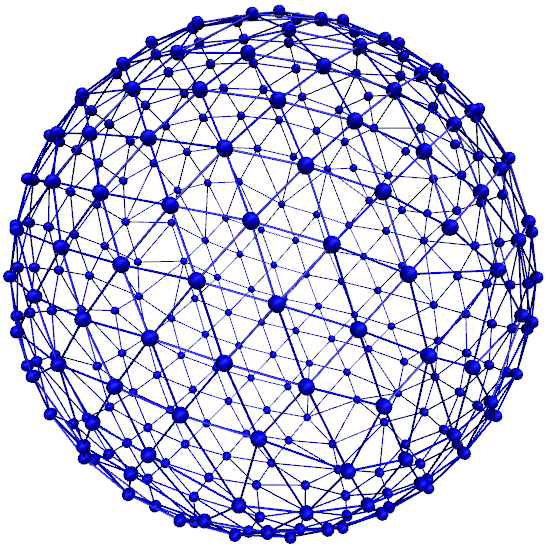
\includegraphics[width=3cm]{figures/fsi.png}
\end{center}
Triangulation can be obtained using various software tools. For mesh input two files are needed:
 \verb mesh-nodes.dat \ and \verb mesh-triangles.dat . The parameters 
of the mesh are the number of particles on the surface of the immersed object, denoted 
by \verb mesh_nnode , and the number of triangular faces in the triangulation, denoted by 
\verb mesh_ntriangle . However, these parameters are obained automatically from 
 \verb mesh-nodes.dat \ and \verb mesh-triangles.dat by counting the number of line in respective files. 

The \verb mesh-nodes.dat \ thus contains \verb mesh_nnode \ lines with three real numbers separated 
by blank space, representing three coordinates of the corresponding particle. The membrane 
is thus discretized into \verb mesh_nnode \ particles with IDs starting from 0 to \verb mesh_nnode-1 . 
The IDs are assigned in the same order as in the \verb mesh-nodes.dat \ file. 

The \verb mesh-triangles.dat \ contains \verb mesh_ntriangle \ lines with three nonnegative 
integers separated by blank space. Each line represents one triangle in the triangulation. 
For algorithmic purposes it is crucial to have defined a correct orientation of the triangle.
The orientation is defined using the normal vector associated with the triangle. The important
 rule is that the normal vector of the triangle must point inside the immersed object.

As an example, let us have one line in the file \verb mesh-triangles.dat \ with numbers 4, 
0 and 7. This means that particles with IDs 4, 0 and 7 form one triangular face of the 
triangulation. The orientation is defined as follows: create two vectors $v_1$ and $v_2$, 
such that $v_1$ is pointing from particle 4 to particle 0, and $v_2$ is pointing from 
particle 4 to particle 7. Be carefull, the order of vectors and particles matters!

The normal vector $n$ is computed as a vector product $v_1 \times v_2$. The direction of 
$n$ can be determined by the rule of right hand: the thumb points in the $v_1$ direction, 
the index finger in the $v_2$ direction and the middle finger in the $n$ direction. 
Following this principle, all the lines in the \verb mesh-triangles.dat \ files must be 
such that the normal vectors of the corresponding triangles must point inside the immersed 
object.

These two files are sufficient to describe the geometry and topology of the triangulation. 
For the definition of bonded interactions the following geometric entities are necessary: 
position of the particles, edges, lengths of the edges,  triangles, areas of triangles, 
angles between two triangles sharing a common edge, surface of the immersed object, 
volume of the immersed object. All these geometrical entities can be computed using the 
information from the files \verb mesh-nodes.dat \ and \verb mesh-triangles.dat \ and the 
computation is done in the script \verb scripts/object_in_fluid.tcl .

The script \verb scripts/object_in_fluid.tcl \  reads 
both mesh files, generates list of edges, and computes all geometrical entities needed for 
definition of bonded interactions. It then executes commands creating the particles, interactions and bonds.
An example of \verb part \ command is as follows:
\begin{verbatim} part 0 pos 3.0 3.0 6.0 type 1 mol 1 mass 1 \end{verbatim}

Note, that there is feature \verb mol \ used for the particles. With this feature we distinguish between different 
objects. The limit for the number of objects is 10000. However it can be increased by changing the 
\verb MAX_OBJECTS_IN_FLUID \ constant. 

Next example shows an interaction.   
\begin{verbatim} inter 106 stretching_force 4.6 5.0 \end{verbatim}
By this command (btw, this command is "invisible for the user, it is execute inside the \verb scripts/object_in_fluid.tcl \ script) an interaction for stretching is created with ID 106. Detailed description of the available types of interactions is presented in Section 
\ref{sec:inter-bonded-fsi}.


%%% Local Variables:
%%% mode: latex
%%% TeX-master: "fsi"
%%% End:
